\documentclass[varwidth=true, border=10pt]{standalone}
\usepackage{tkz-euclide}
\usepackage{tikz}
\usetikzlibrary{patterns}

\begin{document}
\usetkzobj{all}
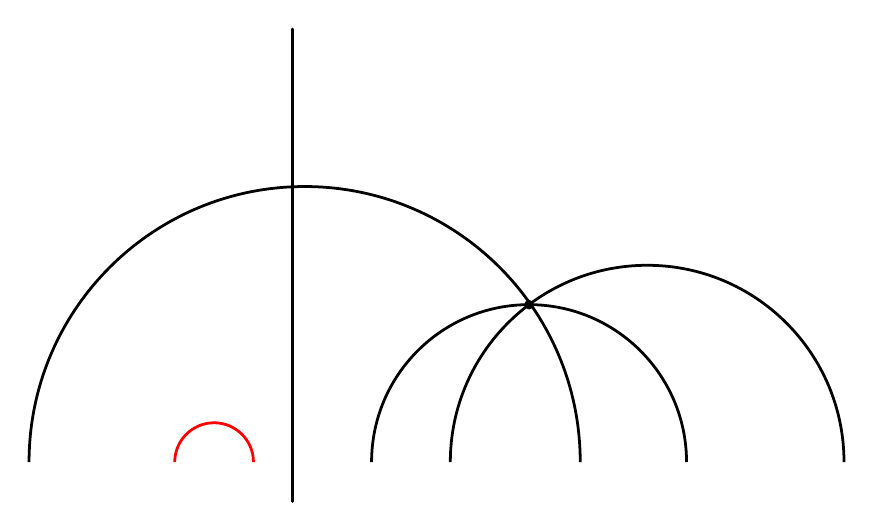
\begin{tikzpicture}
    \tkzSetUpPoint[shape=circle,size=3,color=black,fill=black]
    \tkzSetUpLine[line width=1]
    \tkzInit[xmax=6,ymax=5,xmin=-5,ymin=0]
    \tkzDefPoints{-2/0/A,3.5/0/B,-0.85/0/C,2/0/D,2/2/P}
    \tkzDefPoints{-1/0/X, -1/5/Y}
    \tkzDrawLine[add=0.1 and 0.1](X,Y)
    \tkzAxeXY

    \tkzDrawArc[R,line width=1pt,color=red](A,0.5 cm)(0,180)
    \tkzDrawArc[R,line width=1pt](B,2.5 cm)(0,180)
    \tkzDrawArc[R,line width=1pt](C,3.5 cm)(0,180)
    \tkzDrawArc[R,line width=1pt](D,2.0 cm)(0,180)
    \tkzDrawPoints(P)
\end{tikzpicture}
\end{document}
